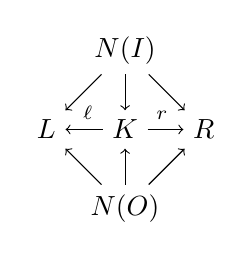
\begin{tikzpicture}
\node (v1) at (0,0) {$L$};
\node (v2) at (1,1) {$N(I)$};
\node (v3) at (1,0) {$K$};
\node (v4) at (1,-1) {$N(O)$};
\node (v5) at (2,0) {$R$};
\draw [->]  
	(v3) edge 
	node [above,pos=0.4] {\scriptsize $\ell$} 
	(v1);
\draw [->] 
	(v3) edge 
	node [above,pos=0.4] {\scriptsize $r$} 
	(v5);
\draw [->] (v2) edge (v1);
\draw [->] (v4) edge (v1);
\draw [->] (v2) edge (v3);
\draw [->] (v4) edge (v3);
\draw [->] (v2) edge (v5);
\draw [->] (v4) edge (v5);
\end{tikzpicture}